\section{On the Use of Categorical and Mixed-Type Features: Analyzing UCI Data}\label{sec:uci}

The following two data sets were obtained from the UCI machine learning repository~\citep{uci}.
Thanks to A. Shapiro, R. Holte and P. Clark for providing the `Chess (King-Rook vs. King-Pawn)' data set of \autoref{subsec:chess},
and to H. Hofmann for providing the `Statlog (German Credit Data)' data set of \autoref{subsec:german}.

%%%%%%%%%%%%%%%%%%%%%%%%%%%%%%%%%%%%%%%%%%%%%%%%%%%%%%%%%%%%%%%%%%%%%%%%%%%%%%%%%%%%%%%%%%%%
\subsection{Chess Data Set --- Illustrating the Use of Categorical Features}\label{subsec:chess}

This data set contains 3196 different board configurations that each describe a starting situation
of the chess endgame `King-Rook versus King-Pawn', in which white has only their
king and pawn left and black has only their king and rook left.
Furthermore it is specified that the white pawn is placed on a7 and white has to make the next move~\citep{shapiro}.
Each of the samples is now the description of one of these scenarios.
In 1669 of the scenarios white is able to win (class 1), the remaining 1527 board configurations will end in a
tie or black will win (class 0).

The 36 nominal raw-text features are statements about the current situation of the game.
These statements are, for example, whether the black king is in the black rook's way (`bklbk'),
or whether the white king is on an edge of the chess board, but not on a8 (`cntxt').
Most of them take the value true (t) or false (f) for each sample, however there are also features with
a more complex behavior like `katri', that states whether the black (b) king, the white (w) king or no (n) king
is in control of the intersect point.
The listing and explanation of all the features can be found in~\cite{shapiro}.

The data set was created by~\cite{shapiro} by generating all possible chess board configurations of a King-Rook versus King-Pawn
endgame and sorting them by a set of characteristics using advanced search algorithms and only considering legal moves.
The main goal is now to find out what characteristics are important to have at the beginning of such
an endgame, in order for the white player to win the game.
The modified SCM is perfect for this task, as it can easily handle the nominal features.

% Performing the algorithm and results

When training the \(SCM_{DNF}\) on all data, it creates the classifier `\texttt{IF (bxqsq=f AND wknck=f AND wkna8=f AND hdchk=f AND spcop=f) OR (rimmx=t) THEN\\won}'.
This corresponds with the feature and base classifier histograms of a cross-validation, as illustrated in \autoref{fig:histChessF}, \autoref{fig:histChessR0} and \autoref{fig:histChessR1}.
In conclusion, and using the interpretations of~\cite{shapiro}, my \(SCM_{DNF}\) classifies the following characteristics
as the essential advantages for the white player to win:

\begin{description}
    \item[rimmx = t:] White can capture the black rook immediately.
    \item[bxqsq = f:] Black does not control a8.
    \item[wknck = f:] The white king is not in check.
    \item[wkna8 = f:] The white king is not in a8.
    \item[hdchk = f:] There is no hidden check. A hidden check would for example happen if the white pawn is on a7, the white king on a5, the black king on a3 and the black rook on a1.
    \item[spcop = f:] There is no special opposition pattern, like white pawn on a7, white king on b8, black king on d7 and black rook on d2, present.
\end{description}

In the studies of~\cite{shapiro} using decision trees, he also came to the conclusion that rimmx and bxqsq are among the most important features.
In many experiments he additionally observed the importance of wknck, wkna8, hdchk and spcop.
However he also notices that the latter features are not really efficient on their own, but shall be used in combination with other:
In the context of decision trees he uses them in subtrees, while I use them as follow-up clauses within a conjunction.

\begin{figure}[H]
    \centering
    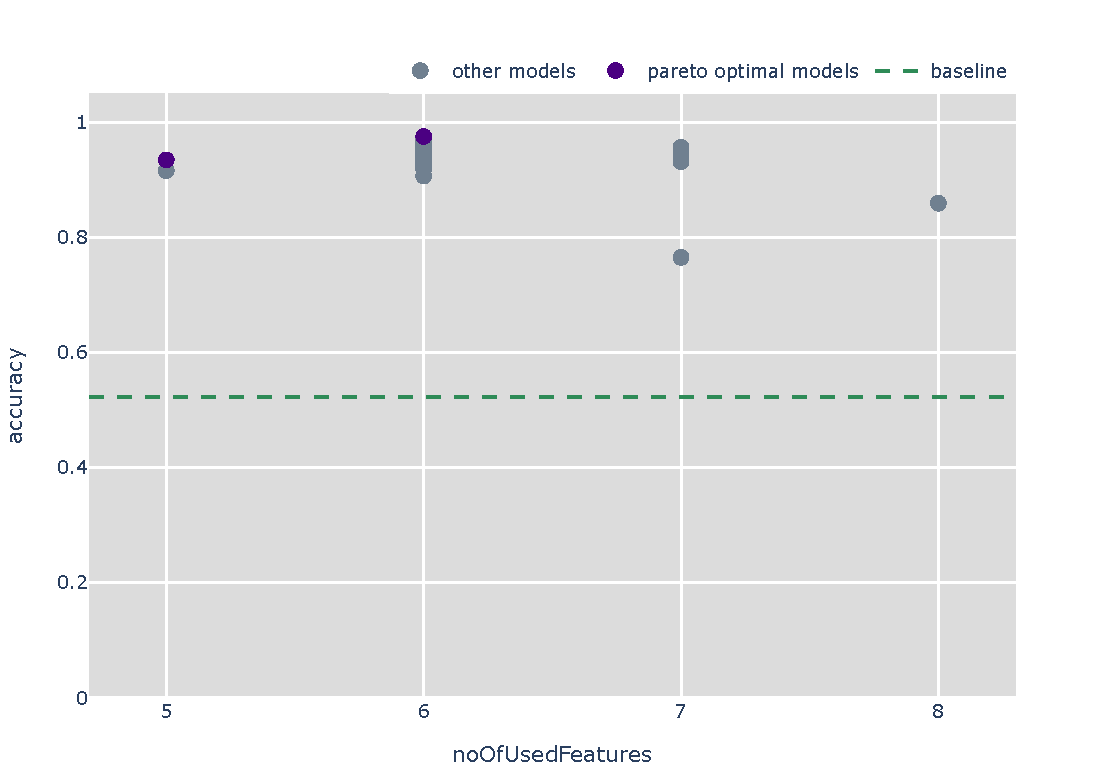
\includegraphics[width=0.85\columnwidth]{figures/chess/paretoFront.pdf}
    \caption{Accuracy-compactness plot for the cross-validation folds of the `chess' data set.}\label{fig:paretoChess}
\end{figure}

With this data set \(p = minConjSize = 1\) was directly usable in order to
obtain good results: in the \(10 \times 10\) cross-validation the \(SCM_{DNF}\) reached a sensitivity of 0.971, a specificity of 0.913
as well as an overall accuracy of 0.943 and therefore a generalization error of only 0.057.
Moreover all 100 models of the cross-validation are located above the baseline (see \autoref{fig:paretoChess}).
In contrast, the \(SCM_{conj}\) only scored an accuracy of 0.809 on the same conditions.
By only using an average of 6.06 features distributed in 2.137 conjunctions per rule, the \(SCM_{DNF}\) is still able to achieve
a good feature compression rate of 83.2\%.

%%%%%%%%%%%%%%%%%%%%%%%%%%%%%%%%%%%%%%%%%%%%%%%%%%%%%%%%%%%%%%%%%%%%%%%%%%%%%%%%%%%%%%%%%%%%
\subsection{German Credit Data --- Illustrating the Use of Mixed-Type Features}\label{subsec:german}

This data set from the Statlog Project contains the data of 1000 applications for a credit in Germany.
700 of these applicants are to be considered as `good' (class 1), the other 300 as `bad' (class 0).
The aim is now to find a rule to classify a new applicant as a good or a bad candidates for a loan, based on their feature values.

As I used the original version of the data set by H. Hofmann, 7 of the 20 features are numerical, like the applicant's age, and 13 are categorical, like purpose of the credit.
Of the categorical features in turn, six are nominal, two binary and therefore handled as nominal and five could be
interpreted as both, ordinal or nominal, so they are treated as nominal.
However, it would certainly be interesting to try and interpret them as ordinal variables in future research.
Additionally the data set is modified by replacing the feature values codes like `A41' with the corresponding real feature values like `car (used)'
from the data set's documentation, so the SCM can produce even more interpretable rules.

The cost matrix, that comes with the data set, implies that the chance of a false positive should be five times lower than the chance of a false negative.
As the chance of a false positive describes the chance that a class 0 samples is classified as class 1, it can be quantified as \(1 - specificity\)
and analog the chance of a false negative equals \(1 - sensitivity\), leading to the requirement of
\[\frac{1-\text{specificity}}{1-\text{sensitivity}} = \frac{1}{5}\]

% Performing the algorithm and results

First of all, different values for \(p\) were tested and the results documented them in \autoref{tab:germanP}.
Here, \(p = \sfrac{3}{7} = \frac{|\text{`negative samples'}|}{|\text{`positive samples'}|}\) was also evaluated, as suggested in \autoref{sec:adjustingParam},
which indeed creates a classifier with a very even sensitivity to specificity ratio.
\(p\) was then gradually decreased until it reached 0.25, at which point the chance of a false negative was
approximately five times higher than the chance of a false positive, fulfilling the data set's requirement.
However, because the data set's classes are very unbalanced, the classifier now only has an accuracy of 0.672,
making it in general even less performant than the trivial classifier `\texttt{IF * THEN good}' with an accuracy of 0.7.

\begin{table}[ht]
    \centering
    \caption{Trying different values for the hyper-parameter \(p\) on the `german' data set.}\label{tab:germanP}
    \begin{tabular}{lllllll}
        \toprule
        \(p\) & acc. \(SCM_{conj}\) & acc. \(SCM_{DNF}\) & |used conj.| & sens. & spec. & \(\frac{1-spec.}{1-sens.}\) \\
        \midrule
        1 & 0.705 & 0.725 & 5.94 & 0.971 & 0.15 & 29.3 \\
        \(\sfrac{4}{7}\) & 0.677 & 0.722 & 9.095 & 0.786 & 0.575 & 1.98 \\
        \(\sfrac{3}{7}\) & 0.669 & 0.672 & 8.545 & 0.667 & 0.698 & \textbf{0.9} \\
        \(\sfrac{2}{7}\) & 0.546 & 0.594 & 8.348 & 0.481 & 0.86 & 0.27 \\
        0.25 & 0.523 & 0.569 & 7.262 & 0.437 & 0.879 & \textbf{0.21} \\
        \bottomrule
    \end{tabular}
\end{table}

The high amounts of used conjunctions per disjunction, depicted in \autoref{tab:germanP},
furthermore indicates that the use of a DNF is indeed helpful for this data set.
Yet it comes with the big trade-off that it increases the size, and therefore the complexity, of the classifier drastically.
This can however be counteracted by increasing the \(minConjSize\).
For \(p=0.25\) the \(SCM_{DNF}\) with \(minConjSize=3\) still has as an accuracy of 0.557
while decreasing the average number of used base classifiers from 18.48 to 11.53 and the number of used conjunctions down to an average of 3.677.

When using the final parameter set of \(p=0.25\) and \(minConjSize = 3\), the resulting
model prefers to give a small credit with a small duration to middle aged people, without
any other installment plans or checking accounts, as portrayed in \autoref{fig:histGermanF} and \autoref{fig:histGermanR1}.
This tendency is also confirmed by the average pareto optimal classifier being
`\texttt{IF (status of existing checking account = no checking account AND\\other installment plans = none
AND age > 22.5 AND credit amount\\< 9504.0 AND age < 66.5) OR (duration in months < 8.5 AND age >\\25.0 AND credit amount < 3015.5)
OR (credit amount < 421.0) THEN good}'.
Additionally \autoref{fig:histGermanR0} provides the insight that 
over 80\% of the classifiers, classify foreign workers to be generally ineligible for a credit.
This is quite shocking, as the data set is only from 1994 and therefore not overly out-of-date.